\documentclass{article}
\usepackage[utf8]{inputenc}
\usepackage{graphicx}
\usepackage{microtype}
\usepackage{subfig}
\usepackage{subfigure}
\usepackage{changepage}
\usepackage{listings}
\usepackage[a4paper,bindingoffset=0.2in,%
            left=1in,right=1in,top=.5in,bottom=.5in,%
            footskip=.25in]{geometry}
\usepackage{titlesec}
\titlelabel{\thetitle.\quad}

\title{Application of Machine Learning in Predicting early marriage in Bangladesh}
\author{Prepared and Presented by \\
Hironmoy paul(21-91902-1) \\ Hedeatul Islam(21-91608-2)\\ Software Documentation and Tools [MScCS] [A]\\ Faculty: Dr. Razib Rayat Khan }
\date{\today}

\begin{document}

\maketitle

\section*{Abstract}
   The early wedding issue has not been tried to be resolved victimization innovative technology of computing. By employing a machine learning technique known as Na Na Bayes classifier, AN early wedding discovered models planned which may be accustomed build a sensible system to detect early wedding potentialities. However, Naive Bias classification is used in police investigation unwellness and the worrying truth early wedding, especially in Bangladesh, has been tried to discover victimization machine learning approach like classification. No correct and effective sensible system is found however to discover an early wedding machine learning approach. That’s why police investigation early wedding or obtaining AN optimum output could be a very crucial and difficult task. different enforced systems that were found are somewhat expensive and unreliable and no detection systems were developed there. however our planned detection model was lightweight weight with less complexness, and that we additionally tested our model on our two hundred inputs of a dataset and found some promising and optimum results. In our planned model, the many issues or determinants of early weddings like education, religion, location, economic condition, etc. are concerned and analyzed. This model can facilitate all the unmated and young ladies with additionally their oldsters to require correct decisions about their valuable life and career.

\section{Introduction}
    A harsh reality of every young woman is marriage before 18. In many parts of the poor and developing countries of the world, young girls are encouraged and forced by their parents to marry in an exceedingly early age when she should go to school and focuses on her study [1]. Several types of machine learning techniques were applied by some authors of India to analyze the cross-sectional survey data as India is covered with a huge number under aged girls who are married as minor, and they are very vulnerable and have the higher risk of many health issues and diseases [6]. Logistic regression, Least Absolute Shrinkage and Selection Operator machine learning techniques were used, and novel and rigorous terms were also applied to get a significant variable grouping related to early marriage [6]. \\\\
    Parent’s ignorance, male dominancy, and social forces etc. diverse types of factors are directly associated for early marriage [2]. Girls in rural areas with poor family background and lower education have elevated risk of early marriage. Early marriage can destroy a girl’s life and hampers her all-basic fundamental rights [2]. Early marriage has a strong correlation with unintentional pregnancy, abortion, child Labor, giving birth of immature babies, immature death due to pregnancy at an early age [2]. Girls who marry at an early age also have psychological disorders and they face a lot of anxiety, depression, and other mood swing disorders. They also face domestic and sexual violence due to early marriage which lead so many girls to immature death. From a report of World Health Organization (WHO), it is found that, 29\% of girls suffer from sexual and physical violence from her husband's [2]. In a survey, 64\% women were found in Bangladesh, who married before 18 years old, and their present ages are between 20 to 24 years old where minimum marriage age for girls is 18 years and 21 years for men [3]. This survey also determines the strong link between lack of education and early marriage. Not only education but also the girls under 18 years old are deprived of their basic rights due to early marriage. As, education has a strong correlation with early marriage, according to the survey, 86\% of women with no education married before 18 years old and the comparatively, 26\% of women completed their secondary and higher education. Location has also a significant link with early marriage. From the early marriage survey, 45\% of women were found who did legal marriage in the rural areas and 55\% of women did legal marriage in urban areas [3]. By delaying marriage extra and immature birth rate can be reduced and controlled [4]. Delaying the first birth, a healthy baby can be born, and the mother can be much fertile [4]. Village people believe that, if they can reduce a member from their family, they can save their households resources by giving marry their Childs [4]. So, financial condition is an important plays a vital role in early marriage. Social violence is also a reason behind early marriage. In rural or village areas, when girls achieve their sexual maturity parents notice their daughters are bullied or teased, then it becomes a big issue for parents and to solve this issue they take the decision of early marriage of their child daughters [5]. So, parents are mainly encouraged to get their children married before 18 years old due to sexual and social norms, family crisis, lower value to daughters and family hardship [5]. When a girl becomes adolescence, her family and society think that he has become a mature woman like others and now she is now capable for marriage, and now she can also have child. These type of thoughts in rural areas, increase the rate of early marriage [5]. 

\section{Literature Review}
    The literature review of this research is divided into three distinct area. Firstly, we introduce Bangladesh to the readers. Secondly, we define the early marriage in the context of Bangladesh. We also present the determinate of early marriage reviewing the latest research. In the third section, we discuss Naïve Bayesian algorithm and its scope of predictability in detecting the determinants of early marriage.\\\\
    Marriage is a union between a man and a woman. It is an interpersonal relationship that is recognize by an official institution, such as the state and church. It is a legal process for a man and a woman to live together in our society. Early marriage is the union of individual people where one or both parties are under 18-year-old. parents in poor families often feel that a young girl is an economic burden to them and therefore they wish to marry off their young girl before they become an economic liability.\\\\
    \textbf{Factors/determinate of early marriage} \\
    \textbf{Education}: Generally, Parents think it would be better to have less educational qualifications for less understanding in family life. That is why they think it is reasonable to get married earlier [2]. \\
    \textbf{Economic Situation}: Poverty is one of the leading causes of early marriage in developing countries. It is said that the cause and effect of marriage can be identified as two. Because parents think girls are an economic burden. And so, marriage is the only reason to fix the economic situation [2]. \\
    \textbf{Culture and customs}: Society has some pre-existing restrictions, behaviors, rules or superstitions. By which parents are still following the rules and marrying girls at an early age. They are marrying girls after their first menstrual period, which can be a source of embarrassment for them [2]. \\
    \textbf{Empirical Review}: There are some social and cultural reasons for child marriage. Such as low-level education of parents, poverty, religion are some of the responsibilities. Girls 'education, girls' living areas are also the reasons for child marriage which is being affected by family income. Family stress and lack of money for education are also the main reasons for child marriage [2].\\\\
    \textbf{What is naïve bias classifier}?\\
    Every collection of classification algorithm based on the Bayes theorem. It is not an individual algorithm but a family of algorithms where they all share a common principle, i.e., each classified feature is distinct from the other. The Naive Bayesian classification is based on the age theorem with assumptions of independence among predictors. Naive Bayes classifier performs surprisingly well and is widely used because it often surpasses more sophisticated classification methods.\\\\
    \textbf{Why do we use naive Bayes classifier}?\\
    Naive Bayes is so fast. it uses the same method to predict the probabilities of different classes based on different characteristics. This algorithm is mostly used in classifying text and with problems in multiple classes. Training is fast because only the probability of each class and the probability of each class of individual input (x) value need to be calculated. No coefficient must be applied in the optimization method.\\
    Here the author mentioned the consequence of early marriage. Like, less education rate, reproductive health issue, miscarriages, domestic violence, quality of marital life, gender equality etc. The author claimed that the schooling and education rate of girls can be increased by more than 20\% if the average age of marriage increases from 15 to 18 years. In every year, dowry accounts for 40\% of extra basic expenses. 0.27\% of unwanted pregnancies can be reduced in every year by delaying the marriage. This paper also has some limitations like lack of mathematical application and implementation [4].\\
    Author has done some surveys according to the year (1993-2011) and in this case it has been seen that the average age of child marriage has increased (14.3-15) from before but slowly. Some of the reasons are low education of husband, wife who is unemployed or not skilled and illiterate etc. The result of this paper is female illiteracy decreased (3\%) and woman education increased (2\%-8\%). Husband education rate is also increasing in this time-period and woman are going to work in huge rate. But unfortunately, unemployment rate is increased in these years. This paper also portrayed some graphical view of some statistical data. The first limitation is that it used cross-sectional and retrospective data sets that might have under-reporting error [7]. \\
    Authors mentioned some evidence of intentional misreporting like variation of ages, current age, age at first marriage, age at first birth. The misleading information was generally collected from older women, less educated woman and most of the households' women. Only 37\% of women are found who accurately mention their real age of marriage. This paper shows that, 90\% of poor people pay dowry where only 45\% of rich people pay dowry. So poor people have the higher tendency for paying dowry. One limitation of this paper is that authors didn’t take any interview of men [8]. \\
    Authors claimed that the girls who get married before 18 years old are likely to be less literate, have many children, have older husband and mostly these girls experience the domestic violence's. So, by increasing the compulsory education of girls, early marriage can be reduced. Early marriage is against of human rights and women have to compromise both of their life and career. To know more about the impact of early marriage on the boys and men, more data collection is needed [1]. \\
    Authors represented a result of the continuous increment of child marriage in Bangladesh. 86\% of women are illiterate and 64\% of women who got married before 18 years old and now their ages are 20 to 24 years old. Authors found a link between area location and early marriage like there is 71\% rate of early marriage in rural area and 54\% rate in urban area. The authors found a limitation that they did not do any research on women's personal decisions in child marriage, thus moving away from women's right to personal opinion [3]. \\
    Two logistic regression model were proposed by authors to get the actual factors related to early marriage. Authors found that women education is inversely dependent on early marriage like women who have secondary education have 45\% less possibility to do early marriage and the women without any primary and secondary education have 9\% less possibility to do early marriage. Mainly this paper focused on women’s education and their partner education, religiosity, possession of health and geographical location which are highly effective to predict early marriage [9]. \\
    The main objective of this research is to find the characteristics of the child marriage victims using database analysis. Based on this research objectives, the research question of this research is: 
    
    \begin{itemize}
        \item What are the characteristics of an individual that influence early child marriage?
    \end{itemize}
    

\section{Proposed Algorithm}


        \subsection{Classifier and formula of naive Bayes}
        The age theorem provides a way to calculate the northern probability, p (c | x), from p (c), p(x) and p (x | c). The Naive Bayes classifier assumes that the effect of the value of a predictor p(x) on a given class p(c) is different from the values of other predictors. This assumption is called class conditional independence. P(c|x) is the antecedent of the prediction (attribute) given by the classified (target). 
        \begin{figure}[!htb]
            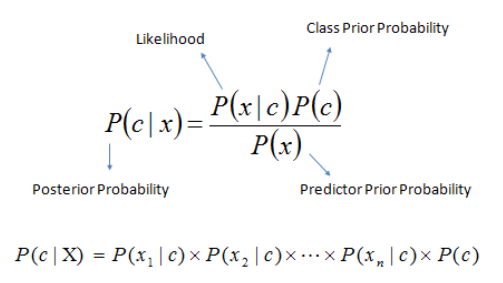
\includegraphics[width=1\textwidth]{Images/naive.png}
        \end{figure} 
        \pagebreak\subsection{Naïve Bias Implementation: }
        In our proposed algorithm, we have applied the Naïve Bayes theorem and all the calculations are done by Naïve Bayes Equation. Some sample calculations and results are given below - 
        \begin{figure}[!htb]
            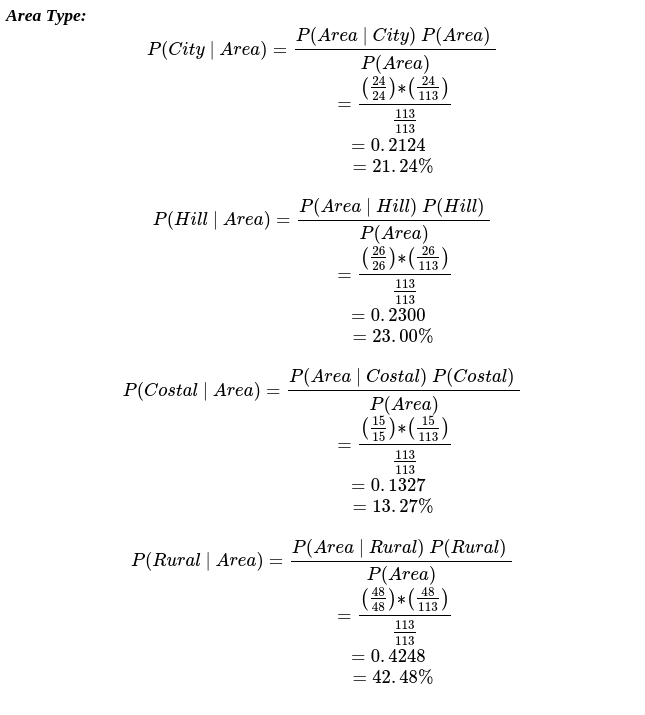
\includegraphics[width=1\textwidth]{Images/area.png}
        \end{figure} 
        \pagebreak\begin{figure}[!htb]
            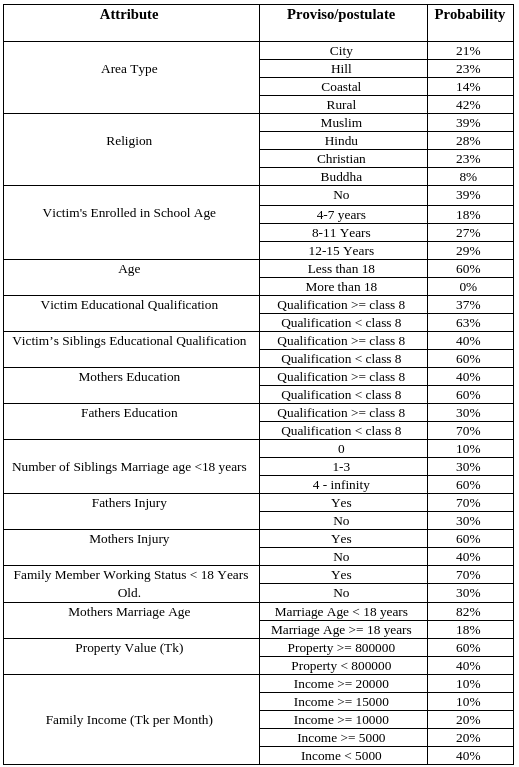
\includegraphics[width=1\textwidth]{Images/table1.png}
            \caption{Data Analysis Table}
        \end{figure} 
 
        \subsection {Description of Proposed Model Table:}
        The causes of early marriage in rural area kind of disobedience and Early marriage as a tribute to ancestors. It is also. Protection of the family's honor. For the reason of poverty Family have Lack of sexual education and unexpected pregnancy. \\
        According to our dataset, we found a variation of early marriage rate depending on area type. 42\% of early marriages occurred in rural areas. In hill areas, 23\% of early marriage rate found, city area has 21\% and coastal areas has 14\% of early marriage rate. According to a research, 70.9\% of child marriage occurred in rural areas and 57\% of child marriage happened in urban areas [1]. \\
        Religion plays a significant role in early marriage. According to our data, we found 39\% of early marriages are occurred in Muslim families. In Hindu religion around 28\% of early marriage are found. Then Christian religion has 23\% rate of early marriage, and the remaining portions are covered by other religions. From a research, it is found that half of the married women are deeply religious and most obedient to their rules and regulations. \\
        Concerning education, more than one-fourth of the married women have no education. 39\% of women who are not enrolled in school and remaining percentage are enrolled in school. According to our dataset, 63\% of women does not have basic primary education, that’s mean they didn’t complete their education of class 8. From our research women school enrolled age 4-7 years 18\%, 8-11 years 27\%, 12-15 years 29\%. Among them only 37\% have basic primary education. Family education is one of key factor of child marriage. If parents are educated, that’s mean they have knowledge to know what is right. Around 65\% of parents who don’t have basic education. Only 40\% of father and 30\% of mother have basic education. That’s why it is also impact of their children. They are not felt to interest to educate their children. 60\% of victim siblings who don’t have basic educational qualifications, according to our dataset. \\
        Siblings' marriage is one of facts of the child marriage. When one or two of the siblings marry at early age, then the whole family follow the trend of early marriage and get all their child married before 18 years old. According to our dataset, 90\% of the siblings who is victim of early marriage. We can also see that 82\% of this family mother is also victim of the early marriage. \\
        There are high chances of early marriage if one's parents are injured. 70\% of child marriage is happened because of their parents' injury and those family have underage workers. Because money is one of the important factors for living this world. If they don’t earn enough money, they can’t buy their necessary livelihood things. Around 70\% of the family have under aged working people. Their property value is under 80k BDT, and they have less amount of monthly income. 40\% of the family have less than 5k BDT Income, 20\% of the family income is around 10K BDT and 10\% of the family income is more than 15k BDT. 

\section{Proposed Model}
    We analyzed several factors and determinants of early marriage and then created a conceptual model which provided an empirical description of this whole research. which is shown the conceptual model and its description are given below - 
    \subsection{Education: }
        Education has a significant impact on early marriage. According to the survey, women with no education married before 18 years. Because of the lack of education, they are not aware of the consequences of early marriage. Because of lack of education girls experience various issues, like have many children, health issue, pregnancy issue etc. They cannot give proper education to their children because of their illiteracy. 
    \subsection{Financial condition: }
        In poor or developing countries, the financial condition of a family has a massive impact on early marriage. If a family financially unstable and has a young girl, the parent feels that the girl is an economic burden to them and tries to marry off their young girl which causes early marriage.
    \subsection{Physical Injury: }
        Sometimes we can say that physical injury is also a cause of early marriage. For example: If the father or mother are injured then the early marriage can happen. Cause they thought if they can marry off their girl's early, they will be the peace of mind. 
    \subsection{Victim:  }
        Victim is called that person who is harmful. From this paper, we can see whose marriage below 18 ages. Those people are called victim. They face several types of problems. Example: Lack of family income, Number of siblings are so high. 
    \subsection{Family marriage:  }
        Family member’s marriage has great impacts on early marriage. Since the father or mother marry at an early age, that’s why they have a high tendency in early marriage with their child daughters also. So that is the reason why early marriage happens. In another issue, sibling marriages has a significant impact on early marriage. When one or two of the siblings marry at early age, then the whole family follow the trend of early marriage and get their child married before 18 years old. Village people believe that, if they can reduce a member from their family, they can save their households resources by giving marry their Childs. 
        \begin{figure}[!htb]
            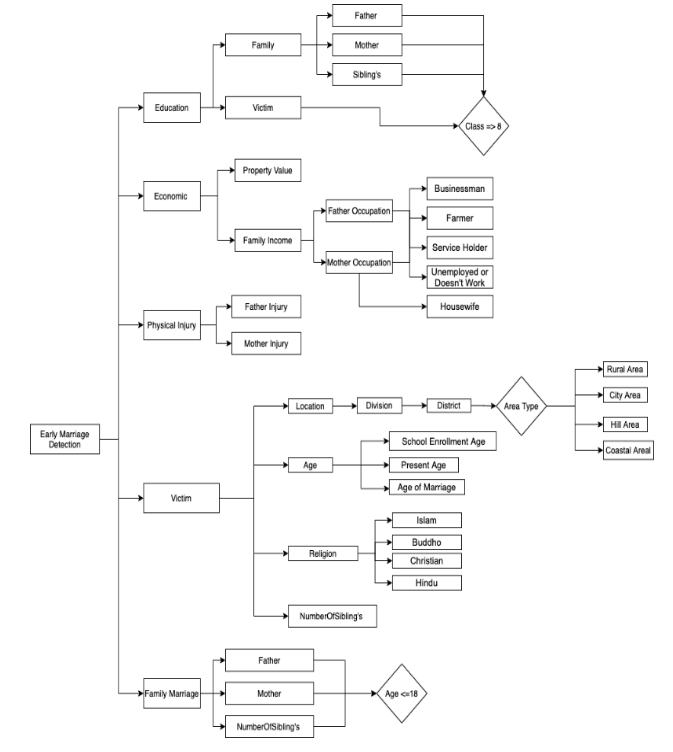
\includegraphics[width=1\textwidth]{Images/figure2.png}
            \caption{Proposed Model}
        \end{figure} 
\pagebreak\section{Conclusion}[!htb]
    This paper provides how to detect early marriage using Naïve Bayes machine learning technique. In the People's Republic of Bangladesh, as early weddings may be a serious social downside, our projected prediction system will with success come through our desired goal. So, this paper shows the associate empirical implementation of machine learning to predict early wedding likelihood betting on some factors like educations, religion, location, condition, etc. during this study, a supervised machine learning technique was applied during a data-set that is collected from a web survey and when analyzing the data-set with our projected technique, we have a tendency to get some best and promising results.
\section{Acknowledgments }
    These should be brief and placed at the end of the text before the references. This example of acknowledgements for a research paper is designed to demonstrate how intellectual, financial and other research contributions should be formally acknowledged in academic and scientific writing. As brief acknowledgements for a research paper, the example gathers contributions of different kinds – intellectual assistance, financial support, image credits etc. – into a single Acknowledgements section. Do note, however, that the formats preferred by some scholarly journals require the separation of certain contributions such as financial support of research into their own sections. \\
    Although authors often write acknowledgements hastily, the Acknowledgements section is an important part of a research paper. Acknowledging assistance and contributions establishes your integrity as a researcher as well as your connections and collaborations. It can also help your readers with their own research, affect the influence and impact of the researchers and other professionals you thank, and demonstrate the value and purpose of the agencies that fund your work. The contents of the example I have prepared here are appropriate for a research paper intended for publication in a peer-reviewed journal, but the author, the research project, the manuscript studied, the journal publishing the paper and all those to whom gratitude is extended are entirely fictional. They were created for the purpose of demonstrating the following key concerns when writing the acknowledgements for a formal research paper 

\begin{thebibliography}{00}
    \bibitem{b1} UNICEF, 2005. Early marriage a harmful traditional practice a statistical exploration 2005. UNICEF. 
    \bibitem{b2} Montazeri, S., Gharacheh, M., Mohammadi, N., Alaghband Rad, J. and Eftekhar Ardabili, H., 2016. Determinants of early marriage from married girls’ perspectives in Iranian setting: a qualitative study. Journal of environmental and public health, 2016. 
    \bibitem{b3} Koenig, M.A., Jamil, K., Streatfield, P.K., Saha, T., Al-Sabir, A., Arifeen, S.E., Hill, K. and Haque, Y., 2007. Maternal health and care-seeking behavior in Bangladesh: findings from a national survey. International family planning perspectives, pp.75-82. 
    \bibitem{b4} Field, E., 2004. Consequences of Early Marriage for women in Bangladesh. draft, October, < efield@ latte. harvard. edu. 
    \bibitem{b5} Chaudhuri, E.R., 2015. Unrecognized sexual abuse and exploitation of children in child, early and forced marriage. Plan International. 
    \bibitem{b6} Raj, A., Dehingia, N., Singh, A., McDougal, L. and McAuley, J., 2020. Application of machine learning to understand child marriage in India. SSM-population health, 12, p.100687. 
    \bibitem{b7} Kamal, S.M., Hassan, C.H., Alam, G.M. and Ying, Y., 2015. Child marriage in Bangladesh: trends and determinants. Journal of biosocial Science, 47(1), p.120. 
    \bibitem{b8} Streatfield, P.K., Kamal, N., Ahsan, K.Z. and Nahar, Q., 2015. Early marriage in Bangladesh: Not as early as it appears. Asian Population Studies, 11(1), pp.94-110. 
    \bibitem{b9} Talukder, A., Hasan, M.M., Razu, S.R. and Hossain, Z., 2020. Early marriage in Bangladesh: a cross-sectional study exploring the associated factors. Journal of international women's studies., 21(1), pp.68-78. 
    \bibitem{b10} Mohammad Bellal Hossain, A. K. M. Nurun Nabi, Ms. Tehmina Ghafur, Md. Aminul Haque, 2017. “CONTEXT OF CHILD MARRIAGE AND ITS IMPLICATIONS IN BANGLADESH.” Department of Population Sciences, University of Dhaka, ISBN: 978-984-34-3399-2 
\end{thebibliography}

\end{document}

